%\usepackage{mathtools}
%\usepackage{commath}
%\usepackage[dvipsnames]{xcolor}
%\usepackage{amsthm}
%\usepackage{graphicx}
\newtheorem{definition}{Definition}
Deep Neural Networks (DNNs) have been instrumental in driving significant
progress in deriving actionable insights from complex input data,
such as videos or images. The primary function of a DNN is to process
input sets, execute iterative computations, and generate outputs aimed
at addressing real-world challenges, including classification, prediction,
and recommendation. However, a notable drawback of these models is
their susceptibility to unpredictable behavior when presented with inputs
markedly different from those encountered during training. Out of distribution
(OOD) input for a DNN comprises data that diverges from
the dataset used in model training, stemming from varying temporal, environmental,
or conditional factors compared to the in-distribution data.
Detecting OOD instances involves determining whether a new sample
aligns with the distribution of known data. There are numerous methods and tools available for detecting OOD inputs \cite{hendrycks2016baseline,ritter2018scalable,abdelzad2019detecting,madras2019detecting}. One such tool discussed and evaluated in this paper is the Sketching Curvature for Out-of-Distribution Detection (SCOD) tool\cite{sharma2021sketching}. This  tool was  jointly developed by Stanford
and MIT, designed to compute an uncertainty metric, $\bf{Unc}(x)$, which is designed to be low when queried on inputs drawn using the probability distribution of the training data, but high for inputs far from this data manifold. A critical component for the OOD analysis using the SCOD tool is establishing a {\bf threshold} value for classifying inputs as OOD, which necessitates knowledge of the probability distribution of the training data or labeled OOD data.  Determining the threshold value for classifying inputs as OOD can be accomplished through diverse methodologies. One approach entail leveraging the probability density function (pdf) of the training data to generate inputs and compute the uncertainty metric using the SCOD tool. However, in practical scenarios, the pdf of the training data is frequently unknown, posing a significant challenge. Another approach entails acquiring labeled inputs from both within and outside the distribution, then using receiver operating characteristic (ROC) analysis to determine the threshold. However, obtaining such labeled data can be challenging in certain scenarios. For example, for Collins's DNN, obtaining these labeled inputs is impractical and costly. Therefore, to address this challenge,  this paper introduces a methodology, which is presented as follows. First, it defines the notion of data similarity and quantifies it using generalization performance parameters $(\delta,\epsilon)$. Second, it computes the performance parameters for data points derived from the training set along with the respective lines connecting these data points. Third, it refines the performance parameter values by utilizing the convex hull of a training dataset of a DNN. Finally, this methodology is illustrated using the ROAAS DNN, and a review of the SCOD tool is provided.

First, the concept of OOD captures the notion that a DNN exhibits high performance when presented with input data similar to the training dataset. However, it may struggle to make accurate decisions when encountering inputs significantly divergent from the training data. Notably, the notion of similarity and dissimilarity is not solely dependent on the dataset but also on the model architecture. For instance, a data point may be considered OOD for one model but within the distribution for another model, even if trained on the same dataset. Hence, it is crucial to formalize not only the notion of proximity in terms of distance but also to capture the sensitivity of the DNN model's weight, as indicated by the SCOD uncertainty metric $\bf{Unc}(x)$. Fig~\ref{fig:Bd} shows two definitions aimed to capture these concepts.
\begin{figure}[ht]
\centering
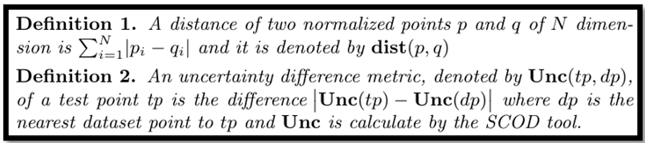
\includegraphics[scale=0.65]{Fig/OOD_def.png}
\caption{Basic definitions.}
\label{fig:Bd}
\end{figure}
With these two definitions, it's feasible to mathematically represent that a test point, tp, is similar to a  training data  if there exists a data point, dp, from the training data such that $\bf{dist}(tp, dp) \leq \delta$ and $\bf{dist}(tp, dp) \leq \epsilon$. The imposition of these two inequalities is essential to prevent scenarios where a test point with a low uncertainty metric is erroneously classified as within the distribution, despite being significantly distant from the training dataset. This rationale motivates the following definition, shown in Fig~\ref{fig:OOD}. 
\begin{figure}[ht]
\centering
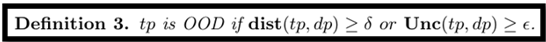
\includegraphics[scale=0.75]{Fig/OOD_def2.png}
\caption{OOD definition.}
\label{fig:OOD}
\end{figure}
These definitions facilitate reframing the task of establishing a threshold value for OOD into the task of determining the generalization performance parameters, $(\delta,\epsilon)$, for managing OOD instances. The computation of these generalization performance parameters is conducted leveraging a DNN model, its associated training dataset, and the SCOD uncertainty metric. This is done next.
 
 
Second, this subsection presents how to calculate $(\delta,\epsilon)$ for data points from the training set and their respective lines between training data points. The computation of the performance parameters occurs through a two-step process, involving the calculation of $\delta$ followed by the computation of $\epsilon$. Initially, $\delta$ is determined as follows: First, for each data point within the training dataset, the closest distance to another data point is computed. Next, $\delta$ is derived as the maximum value among all such closest distances, as illustrated in Fig~\ref{fig:delta}.
\begin{figure}
\centering
\begin{subfigure}{.24\textwidth}
    \centering
    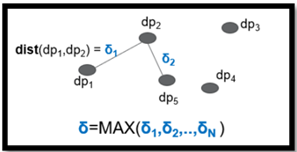
\includegraphics[width=1\linewidth]{Fig/OOD_delta.png}  
    \caption{$\delta$ calculation}
    \label{fig:delta}
\end{subfigure}
\begin{subfigure}{.24\textwidth}
    \centering
    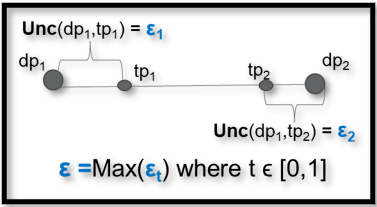
\includegraphics[width=0.93\linewidth]{Fig/OOD_epsilon.png}  
    \caption{$\epsilon$ calculation}
    \label{fig:epsilon}
 \end{subfigure}
\caption{$(\delta,\epsilon)$ calculation}
\label{FIGURE LABEL}
\end{figure}
Next, the computation of $\epsilon$ proceeds as follows: For each data point within the training dataset, a line is generated connecting it to its closest point. Then, for each generated line, the maximum uncertainty difference metric among its constituent points is calculated using the SCOD tool. This process is depicted in Fig~\ref{fig:epsilon}. Ultimately, $\epsilon$ is determined as the maximum uncertainty metric among all generated lines.   Based on the preceding steps, $(\delta,\epsilon)$  could be computed. These generalization performance parameters capture the notion that employing the DNN is deemed safe when a test point either is a training data point (Trivial case) or lies within a line (Reflecting some degree of generalization). However, it's worth noting that the baseline performance parameters  may err on the side of caution. To enhance generalization, the $\delta$ parameter is augmented, a process delineated in the subsequent section.

Third, to further generalize the performance parameters utilizing the $\delta$ parameter, it is necessary to employ a procedure that systematically assesses a set of inputs to identify a subset conducive to generalization. The concept entails leveraging the Operational Design Domain (ODD)\cite{saej3016,torfah2022learning,irvine2021two} as the overarching set, within which a subset conducive to generalization can be identified. 
The ODD within the framework of DNN draws inspiration from autonomous vehicles and robotics. It delineates the specific conditions within which a DNN is engineered and intended to function safely and efficiently. The ODD factors in various considerations, encompassing environmental conditions, temporal aspects, safety constraints, and characteristics of input data. In our pursuit of enhancing the generalization of the performance parameter $\delta$, we will particularly concentrate on the input data characteristics, which entail the distribution and range of features. One methodological approach involves constructing a convex hull within the feature space, represented by the inequality $A.x+b \leq 0$.  The convex hull constitutes the smallest convex set that encompasses all the given points utilized for training. This attribute is pivotal in defining a concise and fundamental set wherein the augmentation of $\delta$ while maintaining $\epsilon$.  In practical terms, we will verify whether the points within the convex hull exhibit a performance parameter $\epsilon$ equivalent to the points along a line, while possessing a larger $\delta$. 
Next subsection illustrate this methodology through an illustrative example.


This last subsection proceeds with the analysis of OOD for the ROAAS model. The primary objective is to obtain the generalization performance parameters using the methodology outlined in the preceding sections. The Runway Overrun Awareness and Alerting System (ROAAS) is a flight deck alerting system providing crews with situational awareness about the possibility of exceeding the end of the runway during aircraft approach and landing. The ROASS DNN model comprises $10$ inputs and $3$ outputs. The objective is to determine the performance parameters 
$(\delta, \epsilon)$ to aid in discerning whether a point is OOD. The computation of these performance parameters unfolds in two steps: the first step involves utilizing a line of the dataset, while the second step entails employing the convex hull of datasets. This phase involves the computation of $\delta$ defined as the maximum of all minimum distances. Fig~\ref{fig:deltaR} posits the value of $\delta$ for ROASS training data. 
\begin{figure}
%\centering
\begin{subfigure}{.24\textwidth}
    %\centering
    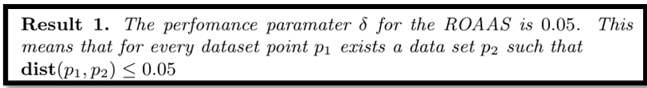
\includegraphics[width=2.0\linewidth]{Fig/OOD_result1.png}  
    \caption{$\delta$ for ROAAS}
    \label{fig:deltaR}
\end{subfigure}
\\
\begin{subfigure}{.24\textwidth}
    %\centering
    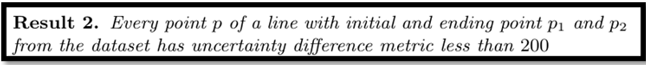
\includegraphics[width=2.0\linewidth]{Fig/OOD_result2.png}  
    \caption{$\epsilon$ for ROAAS}
    \label{fig:epsilonR}
 \end{subfigure}
\caption{$(\delta,\epsilon)$ for ROAAS}
\label{FIGURE LABEL}
\end{figure}
To exemplify this result, consider the data points: $p_1= [8000, 1, 40, 52095, 30, 0,0,0, 161, 0]$ and $p_2= [8000, 1, 40, 52095, 30, 0, 0, 0, 167, 0]$, where the distance between then, denoted by $dist(p_1, p_2)$, equals $0.037$. Subsequently, the calculation of the maximum uncertainty difference metric is executed utilizing the SCOD tool. Fig~\ref{fig:epsilonR} posits the value of $\epsilon$.  To illustrate this result, contemplate the line connecting the data points $dp_1$ and $dp_2$. Each point lying within this line exhibits a performance parameter $\epsilon$ less than $200$, as indicated in Fig~\ref{fig:line}.
\begin{figure}[ht]
\centering
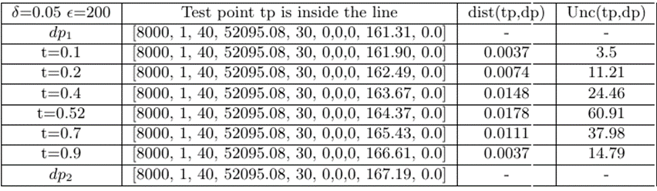
\includegraphics[scale=0.65]{Fig/OOD_result1Exa.png}
\caption{$\epsilon$ for points in a line}
\label{fig:line}
\end{figure}
The baseline values $\delta=0.05$ and $\epsilon=200$ reflect the concept that the model is deemed reliable when the test point either aligns with a training data point (Trivial case) or falls within the line (indicating some degree of generalization). A point is classified as OOD if either its $\epsilon$ exceeds $200$ or its $\delta$ surpasses $0.05$. However, this approach may err on the side of caution. To determine the extent to which we can increase $\delta$, we need a benchmark, and the convex hull serves as our reference point. Our goal is to increase $\delta$ based on the convex hull while ensuring $\epsilon \leq 200$. The convex hull is defined by the equation $A.x+b\leq 0$, where $A$ and $b$ were computed using the ROAAS training dataset. Through random testing, we have formulated a value for $\delta$ as shows Fig~\ref{fig:ConHull}. 
\begin{figure}[ht]
\centering
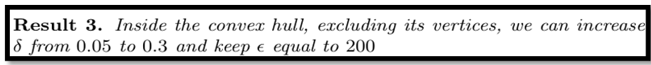
\includegraphics[scale=0.65]{Fig/OOD_result3.png}
\caption{Convex hull}
\label{fig:ConHull}
\end{figure}
Based on this analysis, it is determined that for a ROAAS DNN, a point is considered OOD if either its $\epsilon$ exceeds $200$ or its $\delta$ surpasses $0.3$.



Through the utilization of the SCOD tool for this analysis, the observations suggest that it exhibits a notable degree of adaptability and customization, thereby making it well-suited for a wide spectrum of DNN models. More specifically, it was utilized to compute the $\bf{Unc}$ metric for three Collins's models. Its configurability facilitated the uploading of datasets and DNN models, requiring only minor adjustments such as file format conversions. For instance, public Python libraries were leveraged to convert ONNX models to PyTorch. Although employing ROC analysis to calculate the OOD threshold proved impractical for Collins DNN models, an alternative methodology was devised and implemented as outlined in this paper. Thanks to SCOD's flexibility, integrating the SCOD tool with the Python implementation of this methodology was straightforward, enabling the calculation of generalization performance parameters.